\documentclass[tikz,border=3mm]{standalone}
\usepackage[T1]{fontenc}
\usepackage{lmodern}
\usetikzlibrary{arrows.meta,decorations.pathmorphing}
\begin{document}
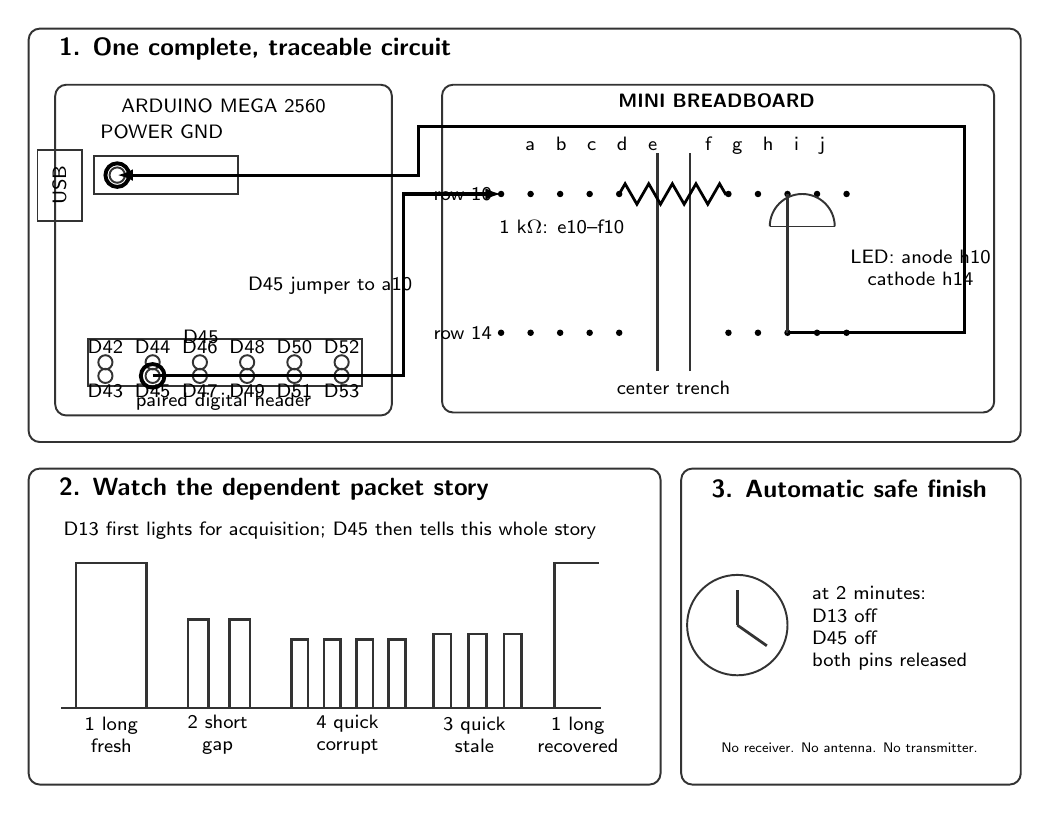
\begin{tikzpicture}[x=0.75cm,y=0.75cm,
  wire/.style={draw=black,line width=1.1pt,-{Latex[length=2mm]}},
  pencil/.style={draw=black!80,line width=.7pt},
  label/.style={font=\sffamily\scriptsize,align=center},
  heading/.style={font=\sffamily\bfseries\small}]

% Panel 1: complete physical circuit.
\draw[pencil,rounded corners] (0,5.8) rectangle (16.8,12.8);
\node[heading,anchor=west] at (.35,12.45)
  {1. One complete, traceable circuit};

% Recognizable Mega geometry and orientation.
\draw[pencil,rounded corners] (.45,6.25) rectangle (6.15,11.85);
\node[label] at (3.3,11.5) {ARDUINO MEGA 2560};
\draw[pencil] (.15,9.55) rectangle (.9,10.75);
\node[label,rotate=90] at (.52,10.15) {USB};
\draw[pencil] (1.0,6.75) rectangle (5.65,7.55);
\node[label] at (3.3,6.48) {paired digital header};
\foreach \x/\top/\bottom in
  {1.3/42/43,2.1/44/45,2.9/46/47,3.7/48/49,4.5/50/51,5.3/52/53}
{
  \draw[pencil] (\x,7.15) circle (.12);
  \draw[pencil] (\x,6.92) circle (.12);
  \node[label] at (\x,7.42) {D\top};
  \node[label] at (\x,6.66) {D\bottom};
}
\draw[black,line width=1.4pt] (2.1,6.92) circle (.2);
\node[label,anchor=south west] at (2.45,7.30) {D45};
\draw[pencil] (1.1,10.0) rectangle (3.55,10.65);
\draw[pencil] (1.5,10.32) circle (.13);
\node[label,anchor=south west] at (1.05,10.78) {POWER GND};
\draw[black,line width=1.4pt] (1.5,10.32) circle (.2);

% Literal mini breadboard: columns a-j, rows 10 and 14, five-hole groups.
\draw[pencil,rounded corners] (7.0,6.3) rectangle (16.35,11.85);
\node[label,font=\sffamily\scriptsize\bfseries] at (11.65,11.58)
  {MINI BREADBOARD};
\node[label] at (10.95,10.82) {a\quad b\quad c\quad d\quad e
  \qquad f\quad g\quad h\quad i\quad j};
\draw[pencil,line width=1pt] (10.65,7.0)--(10.65,10.7);
\draw[pencil,line width=1pt] (11.20,7.0)--(11.20,10.7);
\node[label] at (10.92,6.72) {center trench};
\foreach \y/\row in {10.0/10,7.65/14}
{
  \node[label] at (7.35,\y) {row \row};
  \foreach \x in {8.0,8.5,9.0,9.5,10.0,11.85,12.35,12.85,13.35,13.85}
    \fill (\x,\y) circle (.055);
}

% Complete D45 -> resistor -> LED -> GND net, with exact holes.
\draw[wire] (2.1,6.92) -- (6.35,6.92) -- (6.35,10.0) -- (8.0,10.0);
\node[label,anchor=west] at (3.55,8.45) {D45 jumper to a10};
\draw[black,line width=1pt,decorate,
  decoration={zigzag,segment length=3mm,amplitude=1.3mm}]
  (10.0,10.0)--(11.85,10.0);
\node[label,anchor=east] at (10.25,9.45)
  {1 k$\Omega$: e10--f10};
\draw[pencil,line width=1.2pt] (12.85,10.0)--(12.85,9.45);
\draw[pencil,line width=1.2pt] (12.85,7.65)--(12.85,9.45);
\draw[pencil] (12.55,9.45) arc (180:0:.55 and .55);
\draw[pencil] (12.55,9.45)--(13.65,9.45);
\node[label,anchor=west] at (13.75,8.75)
  {LED: anode h10\\cathode h14};
\draw[wire] (12.85,7.65)--(15.85,7.65)--(15.85,11.15)
  --(6.6,11.15)--(6.6,10.32)--(1.5,10.32);

% Panel 2: dependent visible progression.
\draw[pencil,rounded corners] (0,0) rectangle (10.7,5.35);
\node[heading,anchor=west] at (.35,5.0) {2. Watch the dependent packet story};
\draw[pencil] (.55,1.3)--(9.7,1.3);
\draw[pencil,line width=1pt] (.8,1.3)--(.8,3.75)--(2.0,3.75)--(2.0,1.3);
\draw[pencil,line width=1pt] (2.7,1.3)--(2.7,2.8)--(3.05,2.8)--(3.05,1.3)
  (3.4,1.3)--(3.4,2.8)--(3.75,2.8)--(3.75,1.3);
\foreach \x in {4.45,5.0,5.55,6.1}
  \draw[pencil,line width=1pt] (\x,1.3)--(\x,2.45)--(\x+.28,2.45)--(\x+.28,1.3);
\foreach \x in {6.85,7.45,8.05}
  \draw[pencil,line width=1pt] (\x,1.3)--(\x,2.55)--(\x+.3,2.55)--(\x+.3,1.3);
\draw[pencil,line width=1pt] (8.9,1.3)--(8.9,3.75)--(9.65,3.75);
\node[label] at (1.4,.85) {1 long\\fresh};
\node[label] at (3.2,.85) {2 short\\gap};
\node[label] at (5.4,.85) {4 quick\\corrupt};
\node[label] at (7.55,.85) {3 quick\\stale};
\node[label] at (9.3,.85) {1 long\\recovered};
\node[label] at (5.1,4.3)
  {D13 first lights for acquisition; D45 then tells this whole story};

% Panel 3: automatic shutdown.
\draw[pencil,rounded corners] (11.05,0) rectangle (16.8,5.35);
\node[heading,anchor=west] at (11.4,5.0) {3. Automatic safe finish};
\draw[pencil] (12.0,2.7) circle (.85);
\draw[pencil,line width=1pt] (12.0,2.7)--(12.0,3.3);
\draw[pencil,line width=1pt] (12.0,2.7)--(12.5,2.35);
\node[label,anchor=west] at (13.1,3.25) {at 2 minutes:};
\node[label,anchor=west,align=left] at (13.1,2.45)
  {D13 off\\D45 off\\both pins released};
\node[label,font=\sffamily\tiny] at (13.9,.62)
  {No receiver. No antenna. No transmitter.};
\end{tikzpicture}
\end{document}
